\documentclass[tikz]{standalone}

\usepackage{times}
\usepackage{pgfplots}
\pgfplotsset{compat=1.18}
\usepgfplotslibrary{fillbetween}
% \usepgfplotslibrary{patchplots}

\begin{document}

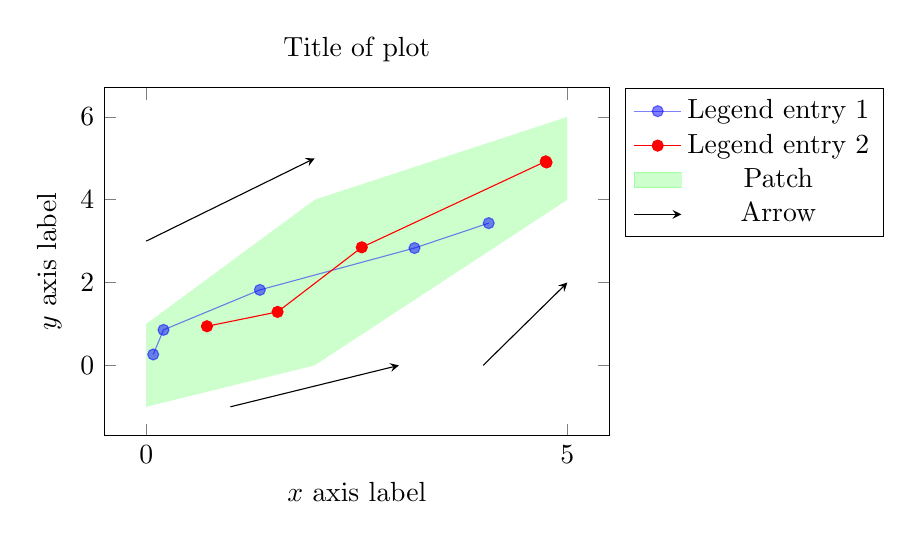
\begin{tikzpicture}
\begin{axis}[
    title={Title of plot},
    xlabel={$x$ axis label},
    ylabel={$y$ axis label},
    % xmin=0,
    % xmax=100,
    % ymin=0,
    % ymax=120,
    % xtick={0, 5},
    % ytick={0, 5},
    xtick distance=5,
    ytick distance=2,
    % xticklabels={,,},
    % yticklabels={,,},
    legend pos=outer north east,
    % legend pos=north west,
    % xmajorgrids=true,
    % ymajorgrids=true,
    % grid style=solid,
    width=8cm,
    height=6cm,
    % width=4cm,
    % height=3cm,
    shader=flat corner,
]

    \addplot[color=blue, mark=*, opacity=0.5]
        coordinates {(0.083,0.263)(0.205,0.857)(1.349,1.822)(3.185,2.833)(4.066,3.434)};
        \addlegendentry{Legend entry 1}

    \addplot[color=red, mark=*, opacity=1]
        coordinates {(0.721,0.944)(1.559,1.291)(2.559,2.850)(4.743,4.926)(4.752,4.899)};
        \addlegendentry{Legend entry 2}

    \addplot[name path=y1, opacity=0, forget plot]
        coordinates{(0,-1)(2,0)(5,4)};

    \addplot[name path=y2, opacity=0, forget plot]
        coordinates{(0,1)(2,4)(5,6)};

    \addplot[green, opacity=0.2]
        fill between[of=y1 and y2];
        \addlegendentry{Patch}

    \addplot[
        quiver={
            u=\thisrow{u},
            v=\thisrow{v},
        },
        -stealth,
    ]
        table {
            x  y  u  v
            1 -1  2  1
            4  0  1  2
            0  3  2  2
        };
        \addlegendentry{Arrow}

    % \addplot[surf]
    %     coordinates{(0.00,4.00,0.00)(0.00,4.40,0.00)(0.00,4.80,0.00)(0.00,5.20,0.00)(0.00,5.60,0.00)(0.00,6.00,0.00)(0.20,4.00,0.80)(0.20,4.40,0.88)(0.20,4.80,0.96)(0.20,5.20,1.04)(0.20,5.60,1.12)(0.20,6.00,1.20)(0.40,4.00,1.60)(0.40,4.40,1.76)(0.40,4.80,1.92)(0.40,5.20,2.08)(0.40,5.60,2.24)(0.40,6.00,2.40)(0.60,4.00,2.40)(0.60,4.40,2.64)(0.60,4.80,2.88)(0.60,5.20,3.12)(0.60,5.60,3.36)(0.60,6.00,3.60)(0.80,4.00,3.20)(0.80,4.40,3.52)(0.80,4.80,3.84)(0.80,5.20,4.16)(0.80,5.60,4.48)(0.80,6.00,4.80)(1.00,4.00,4.00)(1.00,4.40,4.40)(1.00,4.80,4.80)(1.00,5.20,5.20)(1.00,5.60,5.60)(1.00,6.00,6.00)};

    % \addplot [surf,point meta=explicit] coordinates {
    %     (0,0,0) (1,0,1) (2,0,2)  (3,0,3)

    %     (0,1,4) (1,1,5) (2,1,3)  (3,1,7)
    %     (0,2,8) (1,2,9) (2,2,10) (3,2,11)
    % };


\end{axis}
\end{tikzpicture}

\end{document}
